\documentclass{standalone}
\usepackage{tikz}
\usetikzlibrary{patterns, positioning}
\usepackage[sfdefault]{ClearSans} %% option 'sfdefault' activates Clear Sans as the default text font
\usepackage[T1]{fontenc}

\begin{document}
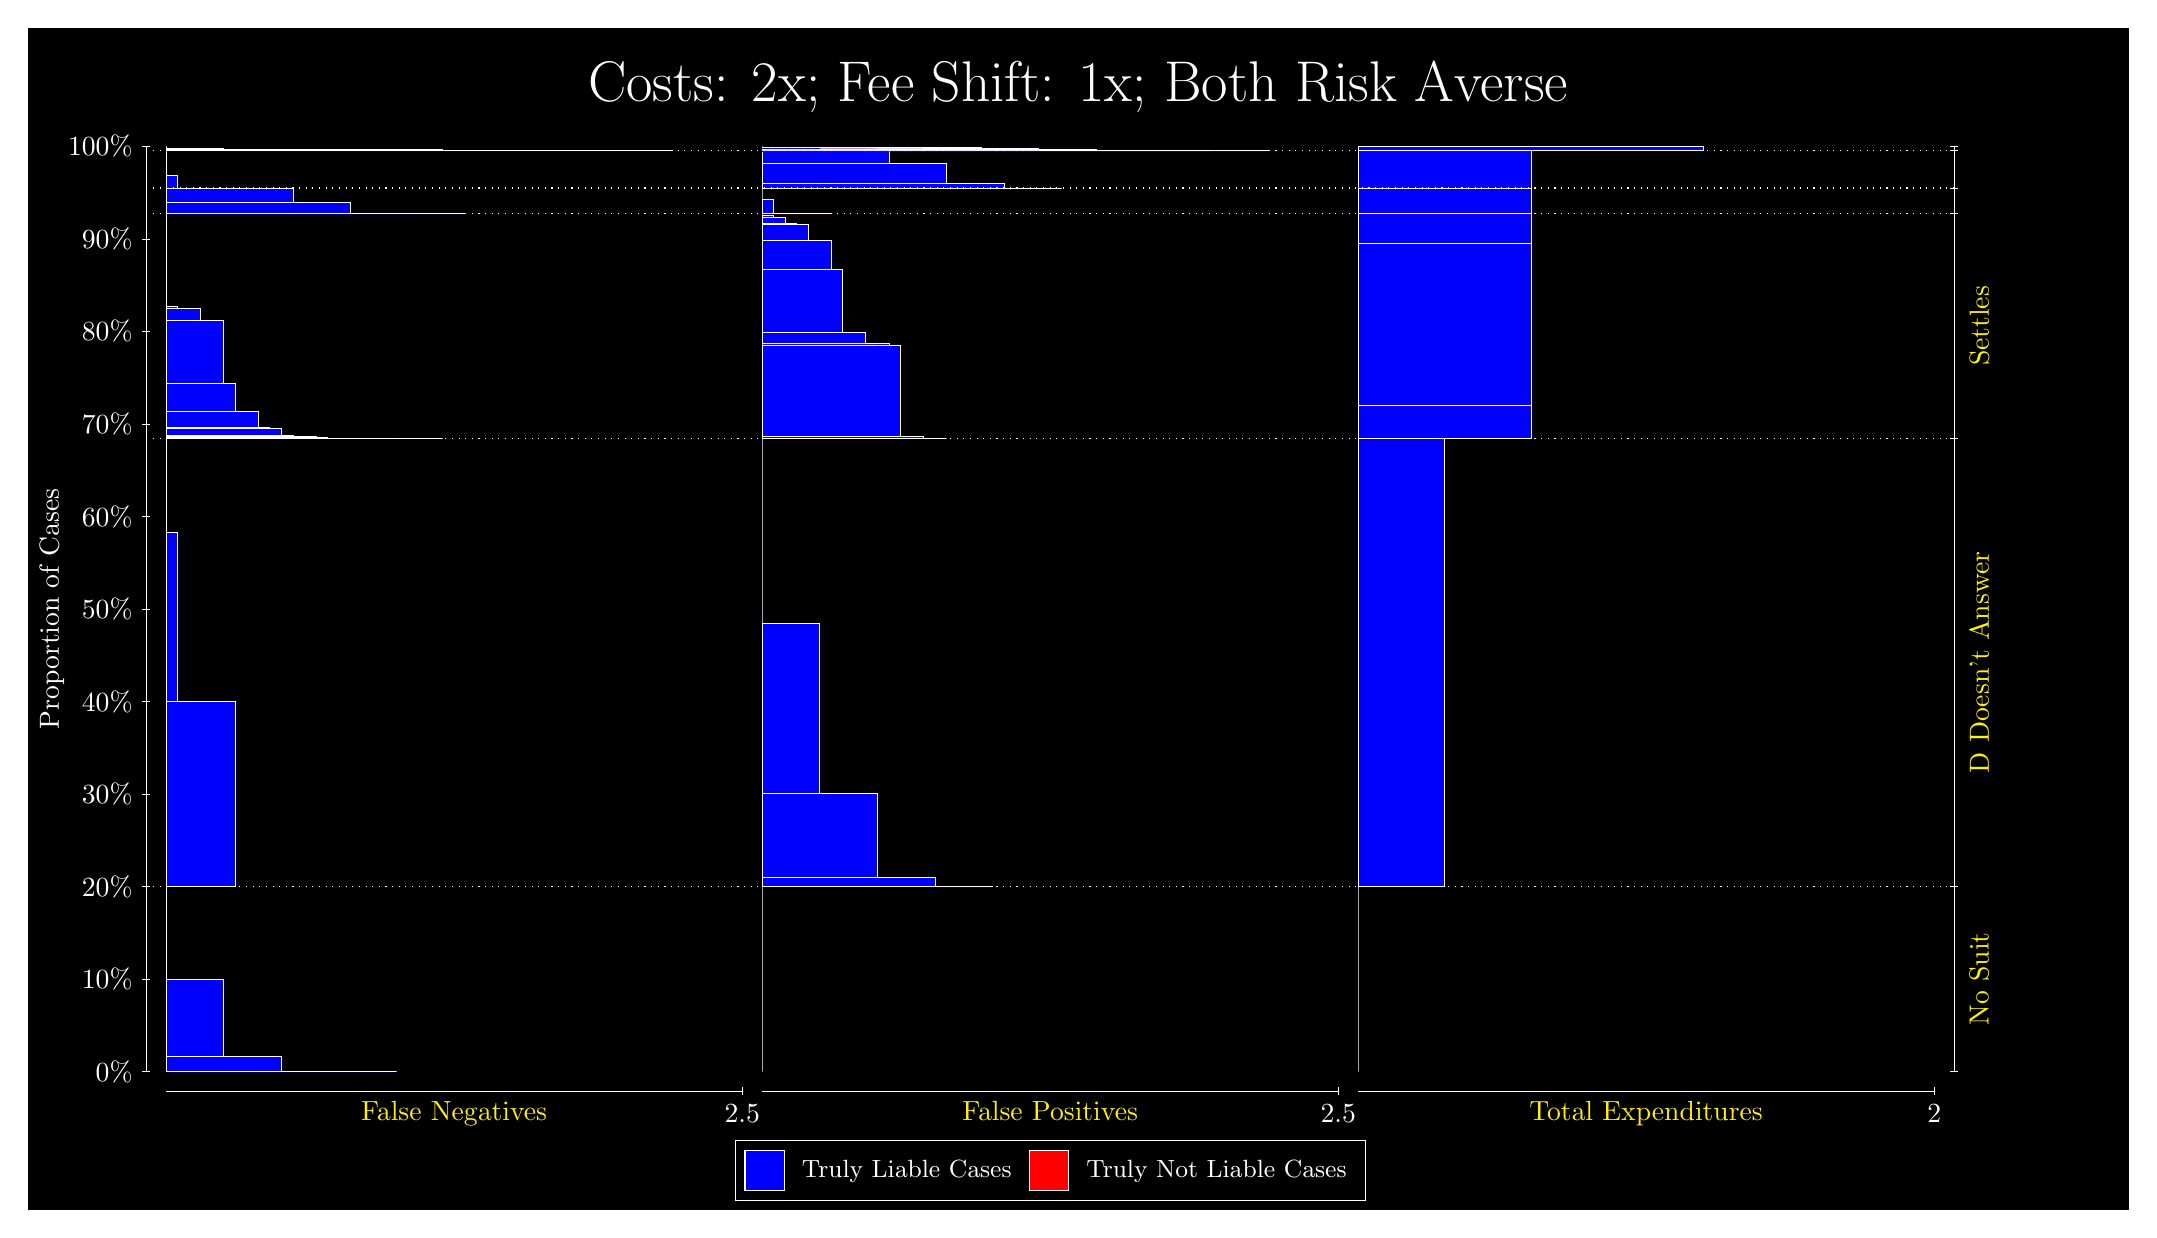
\begin{tikzpicture}
\draw[fill=black] (0,0) rectangle (26.667,15);
\draw[text=white] (0,13.5) rectangle (26.667,15) node[midway] {\huge Costs: 2x; Fee Shift: 1x; Both Risk Averse};
\draw[white, very thin] (1.5,1.75) -- (1.5,13.5);
\node[rotate=90, text=white, anchor=center] at (0.3, 7.625) {Proportion of Cases};
\draw[white, very thin] (1.45,1.75) -- (1.55,1.75);
\node[text=white, anchor=east] at (1.45, 1.75) {0\%};
\draw[white, very thin] (1.45,2.925) -- (1.55,2.925);
\node[text=white, anchor=east] at (1.45, 2.925) {10\%};
\draw[white, very thin] (1.45,4.1) -- (1.55,4.1);
\node[text=white, anchor=east] at (1.45, 4.1) {20\%};
\draw[white, very thin] (1.45,5.275) -- (1.55,5.275);
\node[text=white, anchor=east] at (1.45, 5.275) {30\%};
\draw[white, very thin] (1.45,6.45) -- (1.55,6.45);
\node[text=white, anchor=east] at (1.45, 6.45) {40\%};
\draw[white, very thin] (1.45,7.625) -- (1.55,7.625);
\node[text=white, anchor=east] at (1.45, 7.625) {50\%};
\draw[white, very thin] (1.45,8.8) -- (1.55,8.8);
\node[text=white, anchor=east] at (1.45, 8.8) {60\%};
\draw[white, very thin] (1.45,9.975) -- (1.55,9.975);
\node[text=white, anchor=east] at (1.45, 9.975) {70\%};
\draw[white, very thin] (1.45,11.15) -- (1.55,11.15);
\node[text=white, anchor=east] at (1.45, 11.15) {80\%};
\draw[white, very thin] (1.45,12.325) -- (1.55,12.325);
\node[text=white, anchor=east] at (1.45, 12.325) {90\%};
\draw[white, very thin] (1.45,13.5) -- (1.55,13.5);
\node[text=white, anchor=east] at (1.45, 13.5) {100\%};

\draw[white, very thin] (24.457,1.75) -- (24.457,13.5);
\draw[white, very thin] (24.407,1.75) -- (24.507,1.75);
\node[anchor=west] at (24.407, 1.75) {};
\draw[white, very thin] (24.407,4.0995) -- (24.507,4.0995);
\node[anchor=west] at (24.407, 4.0995) {};
\draw[white, very thin] (24.407,9.7945) -- (24.507,9.7945);
\node[anchor=west] at (24.407, 9.7945) {};
\draw[white, very thin] (24.407,12.646) -- (24.507,12.646);
\node[anchor=west] at (24.407, 12.646) {};
\draw[white, very thin] (24.407,12.971) -- (24.507,12.971);
\node[anchor=west] at (24.407, 12.971) {};
\draw[white, very thin] (24.407,13.446) -- (24.507,13.446);
\node[anchor=west] at (24.407, 13.446) {};
\draw[white, very thin] (24.407,13.5) -- (24.507,13.5);
\node[anchor=west] at (24.407, 13.5) {};

\draw[white, very thin, fill=blue] (1.75,1.75) rectangle (4.6775,1.75);
\draw[white, very thin, fill=blue] (1.75,1.75) rectangle (3.9457,1.7516);
\draw[white, very thin, fill=blue] (1.75,1.7516) rectangle (3.2138,1.938);
\draw[white, very thin, fill=blue] (1.75,1.938) rectangle (2.4819,2.9264);
\draw[white, very thin, fill=red] (1.75,2.9264) rectangle (1.75,2.9264);
\draw[white, very thin, fill=blue] (1.75,2.9264) rectangle (1.75,4.0995);
\draw[white, very thin, fill=blue] (1.75,4.0995) rectangle (2.6283,6.4475);
\draw[white, very thin, fill=blue] (1.75,6.4475) rectangle (1.8964,8.6046);
\draw[white, very thin, fill=red] (1.75,8.6046) rectangle (1.75,8.6046);
\draw[white, very thin, fill=blue] (1.75,8.6046) rectangle (1.75,9.7945);
\draw[white, very thin, fill=blue] (1.75,9.7945) rectangle (5.2631,9.7945);
\draw[white, very thin, fill=blue] (1.75,9.7945) rectangle (4.9703,9.7945);
\draw[white, very thin, fill=blue] (1.75,9.7945) rectangle (4.6775,9.7945);
\draw[white, very thin, fill=blue] (1.75,9.7945) rectangle (4.5312,9.7945);
\draw[white, very thin, fill=blue] (1.75,9.7945) rectangle (4.3848,9.7945);
\draw[white, very thin, fill=blue] (1.75,9.7945) rectangle (4.2384,9.7945);
\draw[white, very thin, fill=blue] (1.75,9.7945) rectangle (4.092,9.7945);
\draw[white, very thin, fill=blue] (1.75,9.7945) rectangle (3.9457,9.7962);
\draw[white, very thin, fill=blue] (1.75,9.7962) rectangle (3.7993,9.8061);
\draw[white, very thin, fill=blue] (1.75,9.8061) rectangle (3.6529,9.8132);
\draw[white, very thin, fill=blue] (1.75,9.8132) rectangle (3.5065,9.8163);
\draw[white, very thin, fill=blue] (1.75,9.8163) rectangle (3.3602,9.8352);
\draw[white, very thin, fill=blue] (1.75,9.8352) rectangle (3.2138,9.9216);
\draw[white, very thin, fill=blue] (1.75,9.9216) rectangle (3.0674,9.9343);
\draw[white, very thin, fill=blue] (1.75,9.9343) rectangle (2.921,10.13);
\draw[white, very thin, fill=blue] (1.75,10.13) rectangle (2.7746,10.133);
\draw[white, very thin, fill=blue] (1.75,10.133) rectangle (2.6283,10.497);
\draw[white, very thin, fill=blue] (1.75,10.497) rectangle (2.4819,11.297);
\draw[white, very thin, fill=blue] (1.75,11.297) rectangle (2.3355,11.297);
\draw[white, very thin, fill=blue] (1.75,11.297) rectangle (2.1891,11.446);
\draw[white, very thin, fill=blue] (1.75,11.446) rectangle (2.0428,11.446);
\draw[white, very thin, fill=blue] (1.75,11.446) rectangle (1.8964,11.473);
\draw[white, very thin, fill=red] (1.75,11.473) rectangle (1.75,11.473);
\draw[white, very thin, fill=blue] (1.75,11.473) rectangle (1.75,12.646);
\draw[white, very thin, fill=blue] (1.75,12.646) rectangle (5.5558,12.646);
\draw[white, very thin, fill=blue] (1.75,12.646) rectangle (4.8239,12.646);
\draw[white, very thin, fill=blue] (1.75,12.646) rectangle (4.092,12.787);
\draw[white, very thin, fill=blue] (1.75,12.787) rectangle (3.3602,12.969);
\draw[white, very thin, fill=blue] (1.75,12.969) rectangle (2.6283,12.971);
\draw[white, very thin, fill=red] (1.75,12.971) rectangle (1.75,12.971);
\draw[white, very thin, fill=blue] (1.75,12.971) rectangle (2.6283,12.973);
\draw[white, very thin, fill=blue] (1.75,12.973) rectangle (1.8964,13.135);
\draw[white, very thin, fill=red] (1.75,13.135) rectangle (1.75,13.135);
\draw[white, very thin, fill=blue] (1.75,13.135) rectangle (1.75,13.446);
\draw[white, very thin, fill=blue] (1.75,13.446) rectangle (8.1906,13.446);
\draw[white, very thin, fill=blue] (1.75,13.446) rectangle (7.4587,13.446);
\draw[white, very thin, fill=blue] (1.75,13.446) rectangle (6.7268,13.447);
\draw[white, very thin, fill=blue] (1.75,13.447) rectangle (5.9949,13.454);
\draw[white, very thin, fill=blue] (1.75,13.454) rectangle (5.2631,13.463);
\draw[white, very thin, fill=blue] (1.75,13.463) rectangle (4.5312,13.463);
\draw[white, very thin, fill=blue] (1.75,13.463) rectangle (3.9457,13.463);
\draw[white, very thin, fill=blue] (1.75,13.463) rectangle (3.7993,13.463);
\draw[white, very thin, fill=blue] (1.75,13.463) rectangle (3.2138,13.463);
\draw[white, very thin, fill=blue] (1.75,13.463) rectangle (2.4819,13.469);
\draw[white, very thin, fill=red] (1.75,13.469) rectangle (1.75,13.469);
\draw[white, very thin, fill=blue] (1.75,13.469) rectangle (1.75,13.5);
\draw[white, very thin, fill=red] (9.3189,1.75) rectangle (9.3189,1.75);
\draw[white, very thin, fill=blue] (9.3189,1.75) rectangle (9.3189,4.0995);
\draw[white, very thin, fill=red] (9.3189,4.0995) rectangle (12.246,4.0995);
\draw[white, very thin, fill=blue] (9.3189,4.0995) rectangle (12.246,4.1005);
\draw[white, very thin, fill=blue] (9.3189,4.1005) rectangle (11.515,4.2147);
\draw[white, very thin, fill=blue] (9.3189,4.2147) rectangle (10.783,5.2894);
\draw[white, very thin, fill=blue] (9.3189,5.2894) rectangle (10.051,7.4465);
\draw[white, very thin, fill=blue] (9.3189,7.4465) rectangle (9.3189,9.7945);
\draw[white, very thin, fill=red] (9.3189,9.7945) rectangle (11.661,9.7945);
\draw[white, very thin, fill=blue] (9.3189,9.7945) rectangle (11.661,9.7945);
\draw[white, very thin, fill=red] (9.3189,9.7945) rectangle (11.368,9.7945);
\draw[white, very thin, fill=blue] (9.3189,9.7945) rectangle (11.368,9.8172);
\draw[white, very thin, fill=red] (9.3189,9.8172) rectangle (11.075,9.8172);
\draw[white, very thin, fill=blue] (9.3189,9.8172) rectangle (11.075,10.967);
\draw[white, very thin, fill=blue] (9.3189,10.967) rectangle (10.929,10.994);
\draw[white, very thin, fill=red] (9.3189,10.994) rectangle (10.783,10.994);
\draw[white, very thin, fill=blue] (9.3189,10.994) rectangle (10.783,10.994);
\draw[white, very thin, fill=blue] (9.3189,10.994) rectangle (10.636,11.143);
\draw[white, very thin, fill=red] (9.3189,11.143) rectangle (10.49,11.143);
\draw[white, very thin, fill=blue] (9.3189,11.143) rectangle (10.49,11.143);
\draw[white, very thin, fill=blue] (9.3189,11.143) rectangle (10.344,11.943);
\draw[white, very thin, fill=blue] (9.3189,11.943) rectangle (10.197,12.307);
\draw[white, very thin, fill=blue] (9.3189,12.307) rectangle (10.051,12.31);
\draw[white, very thin, fill=blue] (9.3189,12.31) rectangle (9.9044,12.506);
\draw[white, very thin, fill=blue] (9.3189,12.506) rectangle (9.758,12.519);
\draw[white, very thin, fill=blue] (9.3189,12.519) rectangle (9.6116,12.605);
\draw[white, very thin, fill=blue] (9.3189,12.605) rectangle (9.4652,12.624);
\draw[white, very thin, fill=blue] (9.3189,12.624) rectangle (9.3189,12.646);
\draw[white, very thin, fill=red] (9.3189,12.646) rectangle (10.197,12.646);
\draw[white, very thin, fill=blue] (9.3189,12.646) rectangle (10.197,12.648);
\draw[white, very thin, fill=blue] (9.3189,12.648) rectangle (9.4652,12.83);
\draw[white, very thin, fill=blue] (9.3189,12.83) rectangle (9.3189,12.971);
\draw[white, very thin, fill=red] (9.3189,12.971) rectangle (13.125,12.971);
\draw[white, very thin, fill=blue] (9.3189,12.971) rectangle (13.125,12.971);
\draw[white, very thin, fill=blue] (9.3189,12.971) rectangle (12.393,13.032);
\draw[white, very thin, fill=blue] (9.3189,13.032) rectangle (11.661,13.283);
\draw[white, very thin, fill=blue] (9.3189,13.283) rectangle (10.929,13.445);
\draw[white, very thin, fill=blue] (9.3189,13.445) rectangle (10.197,13.446);
\draw[white, very thin, fill=red] (9.3189,13.446) rectangle (15.759,13.446);
\draw[white, very thin, fill=blue] (9.3189,13.446) rectangle (15.759,13.446);
\draw[white, very thin, fill=blue] (9.3189,13.446) rectangle (15.028,13.446);
\draw[white, very thin, fill=red] (9.3189,13.446) rectangle (15.028,13.446);
\draw[white, very thin, fill=blue] (9.3189,13.446) rectangle (15.028,13.446);
\draw[white, very thin, fill=blue] (9.3189,13.446) rectangle (14.296,13.447);
\draw[white, very thin, fill=red] (9.3189,13.447) rectangle (14.296,13.447);
\draw[white, very thin, fill=blue] (9.3189,13.447) rectangle (14.296,13.448);
\draw[white, very thin, fill=blue] (9.3189,13.448) rectangle (13.564,13.448);
\draw[white, very thin, fill=red] (9.3189,13.448) rectangle (13.564,13.448);
\draw[white, very thin, fill=blue] (9.3189,13.448) rectangle (13.564,13.459);
\draw[white, very thin, fill=blue] (9.3189,13.459) rectangle (12.832,13.459);
\draw[white, very thin, fill=blue] (9.3189,13.459) rectangle (12.832,13.477);
\draw[white, very thin, fill=blue] (9.3189,13.477) rectangle (12.1,13.483);
\draw[white, very thin, fill=blue] (9.3189,13.483) rectangle (11.368,13.483);
\draw[white, very thin, fill=red] (9.3189,13.483) rectangle (10.783,13.483);
\draw[white, very thin, fill=blue] (9.3189,13.483) rectangle (10.783,13.483);
\draw[white, very thin, fill=blue] (9.3189,13.483) rectangle (10.636,13.483);
\draw[white, very thin, fill=red] (9.3189,13.483) rectangle (10.051,13.483);
\draw[white, very thin, fill=blue] (9.3189,13.483) rectangle (10.051,13.484);
\draw[white, very thin, fill=red] (9.3189,13.484) rectangle (9.3189,13.484);
\draw[white, very thin, fill=blue] (9.3189,13.484) rectangle (9.3189,13.5);
\draw[white, very thin, fill=red] (16.888,1.75) rectangle (16.888,1.75);
\draw[white, very thin, fill=blue] (16.888,1.75) rectangle (16.888,4.0995);
\draw[white, very thin, fill=red] (16.888,4.0995) rectangle (17.986,4.0995);
\draw[white, very thin, fill=blue] (16.888,4.0995) rectangle (17.986,9.7945);
\draw[white, very thin, fill=red] (16.888,9.7945) rectangle (19.083,9.7945);
\draw[white, very thin, fill=blue] (16.888,9.7945) rectangle (19.083,10.205);
\draw[white, very thin, fill=red] (16.888,10.205) rectangle (19.083,10.205);
\draw[white, very thin, fill=blue] (16.888,10.205) rectangle (19.083,12.272);
\draw[white, very thin, fill=red] (16.888,12.272) rectangle (19.083,12.272);
\draw[white, very thin, fill=blue] (16.888,12.272) rectangle (19.083,12.646);
\draw[white, very thin, fill=red] (16.888,12.646) rectangle (19.083,12.646);
\draw[white, very thin, fill=blue] (16.888,12.646) rectangle (19.083,12.971);
\draw[white, very thin, fill=red] (16.888,12.971) rectangle (19.083,12.971);
\draw[white, very thin, fill=blue] (16.888,12.971) rectangle (19.083,13.446);
\draw[white, very thin, fill=red] (16.888,13.446) rectangle (21.279,13.446);
\draw[white, very thin, fill=blue] (16.888,13.446) rectangle (21.279,13.448);
\draw[white, very thin, fill=red] (16.888,13.448) rectangle (21.279,13.448);
\draw[white, very thin, fill=blue] (16.888,13.448) rectangle (21.279,13.5);
\draw[white, dotted] (1.5,4.0995) -- (24.457,4.0995);
\draw[white, dotted] (1.5,9.7945) -- (24.457,9.7945);
\draw[white, dotted] (1.5,12.646) -- (24.457,12.646);
\draw[white, dotted] (1.5,12.971) -- (24.457,12.971);
\draw[white, dotted] (1.5,13.446) -- (24.457,13.446);
\draw[white, very thin] (1.75,1.5) -- (9.0689,1.5);
\node[text=yellow, anchor=north] at (5.4094, 1.5) {False Negatives};
\draw[white, very thin] (9.0689,1.45) -- (9.0689,1.55);
\node[text=white, anchor=north] at (9.0689, 1.45) {2.5};

\draw[white, very thin] (9.3189,1.5) -- (16.638,1.5);
\node[text=yellow, anchor=north] at (12.978, 1.5) {False Positives};
\draw[white, very thin] (16.638,1.45) -- (16.638,1.55);
\node[text=white, anchor=north] at (16.638, 1.45) {2.5};

\draw[white, very thin] (16.888,1.5) -- (24.207,1.5);
\node[text=yellow, anchor=north] at (20.547, 1.5) {Total Expenditures};
\draw[white, very thin] (24.207,1.45) -- (24.207,1.55);
\node[text=white, anchor=north] at (24.207, 1.45) {2};

\node[text=yellow, centered, rotate=90] at (24.777, 2.9247) {No Suit};
\node[text=yellow, centered, rotate=90] at (24.777, 6.947) {D Doesn't Answer};
\node[text=yellow, centered, rotate=90] at (24.777, 11.22) {Settles};




\draw (12.978300999999998,1.5) node[draw=none] (baseCoordinate) {};
\begin{scope}[align=center]
        \matrix[scale=0.5, draw=white, below=0.5cm of baseCoordinate, nodes={draw}, column sep=0.1cm]{
            \node[rectangle, draw, minimum width=0.5cm, minimum height=0.5cm, fill=blue] {}; &
            \node[draw=none, font=\small, text=white] (B) {Truly Liable Cases}; &
            \node[rectangle, draw, minimum width=0.5cm, minimum height=0.5cm, fill=red] {}; &
            \node[draw=none, font=\small, text=white] (B) {Truly Not Liable Cases}; \\
            };
\end{scope}

\end{tikzpicture}
\end{document}